\section{Baza podataka}

\subsection{Tabele}

\textbf{Zaposleni:}
Informacije o osoblju firme: menadžeri,komercijalisti,knjigovodje,
\newline
magacioneri i vozači.
\newline
\textbf{Kupci i Dobavljači:}
Informacije poslovnim partnerima. Dobavljač moze biti i kupac, i obratno.
\newline
\textbf{Kontakt osoba:}
Pojedinci tj. zaposleni kod kupca ili dobavljača, sa kojima imamo kontakt, i sa kojima sklapamo posao.
\newline
\textbf{Dokument:}
Predstavlja generalizaciju porudžbina,narudžbina,ponuda,
\newline
otpremnica,prijemnica,faktura,popis. Izradjuju ih zaposleni. Svaki dokument sadrzi stavke, koje sadrze proizvod i njegovu količinu.
\newline
\textbf{Izradjuje:}
Informacije koji zaposleni učestvuje u izradi kog dokumenta.
\newline
\textbf{Porudžbine i Narudžbine:}
Specijalizacija dokumenta, samim tim sadrže i stavke, pored sebi svojstvenih podataka.
\newline
\textbf{Ponuda:}
Specijalizacija dokumenta, samim tim sadrži i stavke, pored sebi svojstvenih podataka. Ponuda je vezana za porudžbinu, koja moze imati vise ponuda.
\newline
\textbf{Otpremnice i Prijemnice:}
Specijalizacija dokumenta, samim tim sadrže i stavke, pored sebi svojstvenih podataka. Vezane za ponudu, koja moze imati više otpremnica i prijemnica.
\newline
\textbf{FaktureUlaz:}
Specijalizacija dokumenta, samim tim sadrže i stavke, pored sebi svojstvenih podataka. Vezane za otpremnicu, za jednu otpremnica postoji jedna faktura.
\newline
\textbf{FaktureIzlaz:}
Specijalizacija dokumenta, samim tim sadrze i stavke, pored sebi svojstvenih podataka. Vezane za prijemnicu, za jednu prijemnicu postoji jedna faktura.
\newline
\textbf{Resursi firme:}
Informacije o materijalnom vlasništvu firme. Zaduzuju ih zaposleni, koji su evidentirani u tabeli \textbf{Zaposleni\_has\_ResursFirme}.
\newline
\textbf{Proizvod:}
Informacije o proizvodima koje firma prodaje. Mogu se kombinovati u nove proizvode, recimo u slucaju akcija ili posebnih ponuda. To je prikazano u tabeli \textbf{Proizvod\_has\_Proizvod}.
\newline
\textbf{Stavka:}
Ucestvuje u svim dokumentima, prikazuje koje proizvode ti dokumenti sadrze.
\newline
\textbf{Magacin:}
Informacije o magacinu, broj vozila ,broj zaposlenih.
\textbf{Popis:}
Specijalizacija dokumenta, kreiraju je magacioneri. Prikazuje viškove i manjkove u magacinu.

\begin{figure}[ht]
\centering
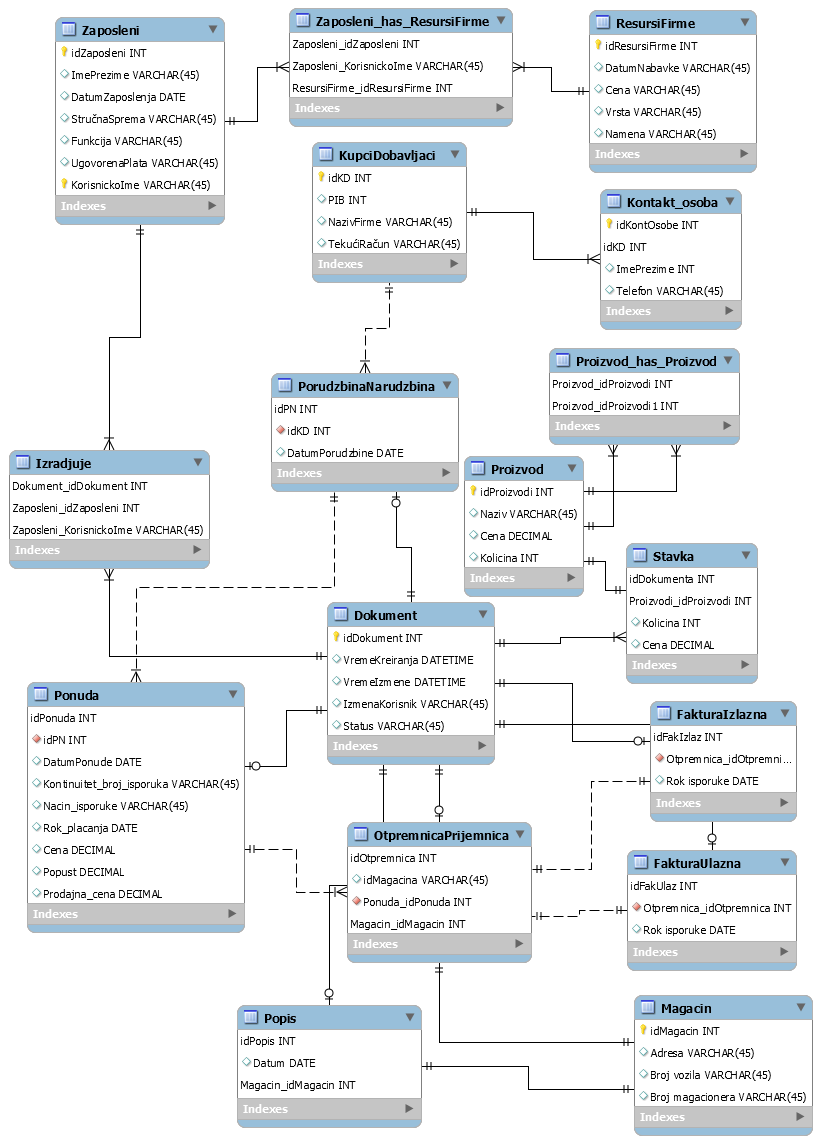
\includegraphics[width=165mm]{slike/er_diagram.png}%
\caption{DTP nivoa 0}
\end{figure}

\clearpage